\documentclass[12pt,addpoints,answers]{evalua}
\grado{3$^\circ$ de Secundaria}
\cicloescolar{2025-2026}
\materia{Olimpiada de Conocimientos 2026}
\unidad{1}
\title{Propuesta para Examen}
\aprendizajes{\item x}
\author{Profesores de Secundaria}
\begin{document}
% \begin{multicols}{2}
	\tableofcontents
% \end{multicols}%\newpage
\begin{questions}\large
		\section{Lenjuages}
                \subsection{Lengua Materna}
                \question[5]{¿Cuál es la función de las convocatorias?
    \begin{choices}
        \choice Expresar sentimientos íntimos del autor a través de versos y estrofas.
        \CorrectChoice Invitar a participar en un evento o concurso.
        \choice Informar de manera objetiva sobre un acontecimiento reciente.
        \choice Entablar una conversación informal entre dos amigos lejanos.
    \end{choices}
                }

    \question[5]{¿Cuáles son dos características de los textos literarios?
    \begin{choices}
        \choice Cuentan con un título, introducción, desarrollo, conclusión y fuentes de consulta.
        \CorrectChoice Se emplean en cartas y funcionan como una técnica de discusión donde se exponen ideas y puntos de vista fundamentados.
        \choice Son textos breves que narran una historia de principio a fin de forma muy rápida.
        \choice Su única finalidad es convocar a personas a un evento público.
    \end{choices}
    }

    \question[5]{¿Cuáles son las partes que conforman un artículo informativo?
    \begin{choices}
        \choice Inicio, nudo, clímax y desenlace.
        \choice Remitente, destinatario, saludo y despedida.
        \CorrectChoice Título, introducción, desarrollo, conclusión y fuentes de consulta.
        \choice Verso, estrofa, rima y métrica.
    \end{choices}
    }

    \question[5]{¿A qué se le llama micorrelatos?
    \begin{choices}
        \choice A las obras teatrales divididas en tres actos o jornadas.
        \choice A los artículos de opinión publicados en los periódicos.
        \CorrectChoice A los textos narrativos que cuentan una historia de principio a fin.
        \choice A los textos formales que se envían a un destinatario específico.
    \end{choices}
}
    \question[5]{¿Qué son las cartas o epístolas?
    \begin{choices}
        \choice Textos que sirven exclusivamente para invitar a concursos.
        \CorrectChoice Son textos formales o personales en los que un remitente entabla comunicación con un destinatario específico.
        \choice Textos narrativos breves que contienen un inicio y un desenlace rápido.
        \choice Artículos cuyo objetivo es mostrar fuentes de consulta sobre un tema.
    \end{choices}
    }

    \subsection{Inglés}
    \question[5]{What presents did you \underline{\hspace{2cm}} for your last birthday?
    \begin{choices}
        \choice will receive
        \CorrectChoice receive
        \choice receiving
        \choice received
    \end{choices}
}

    \question[5]{We use ``someone'', ``anyone'' and ``no one'' to talk about:
    \begin{choices}
        \CorrectChoice people
        \choice locations
        \choice things
        \choice numbers
    \end{choices}
    }
    \vspace{0.3cm}

    \question[5]{I think \underline{\hspace{2cm}} is the most serious crime. Killing someone is unacceptable.
    \begin{choices}
        \choice pickpocketing
        \choice vandalism
        \choice theft
        \CorrectChoice murder
    \end{choices}
   }

    \question[5]{We have the same taste in music, so we always \underline{\hspace{2cm}} which bands are the best.
    \begin{choices}
        \choice worry about
        \choice wait for
        \choice argue with
        \CorrectChoice agree about
    \end{choices}
   }

    \question[5]{This soup tastes horrible - I should have used a better \underline{\hspace{2cm}}.
    \begin{choices}
        \choice article
        \CorrectChoice recipe
        \choice advertisement
        \choice receipt
    \end{choices}
    }

    	\section{Saberes y pensamiento científico}
\subsection{Matemáticas}

\question[5]{Usando la función trigonométrica correcta, encuentra el valor de los lados $x$, para cada uno de los siguientes ejercicios:

    \begin{multicols}{2}

        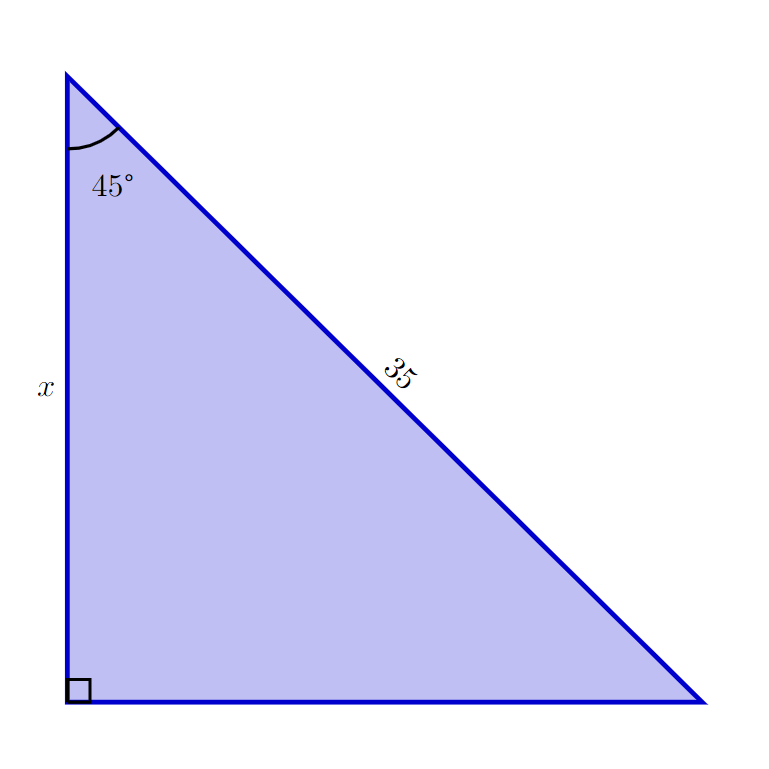
\includegraphics[width=0.9\linewidth]{images/mex_0091.png}

        \begin{solutionbox}{7cm}
            $x=$\fillin[$37.08$][0cm]
        \end{solutionbox}

        % \part 
\includegraphics[width=0.9\linewidth]{mex_0092.png}

        % \begin{solutionbox}{5cm}
        %     $x=$\fillin[$24.84$][0cm]
        % \end{solutionbox}
    \end{multicols}
}

\question[5]{Resuelve el siguiente sistema de ecuaciones lineales:

            \begin{align*}
                  x + 2y +3z  & = 12 \\
                  x - 3y +4z  & = 27 \\
                  -x +  y +2z & = 7
            \end{align*}

            \begin{solutionbox}{8cm}
            \end{solutionbox}
      }

      \question[5]{La suma de dos números es 215 y el mayor excede al menor en 31 unidades. ¿Cuáles son estos dos números?}
 
%       \begin{choices}
%         \choice
%         \CorrectChoice
%         \choice
%         \choice
%     \end{choices}
    

      \subsection{Química}
\section{De lo Humano a lo comunitario}
\subsection{Informática}
 	\question[5]{¿Qué es una hoja de cálculo y para qué sirve?
    \begin{choices}
        \choice Es un procesador de textos diseñado para redactar cartas, memorándums y documentos formales de oficina.
        \CorrectChoice Es una herramienta digital que permite organizar, calcular y analizar información mediante tablas, filas y columnas, utilizada para operaciones matemáticas, registros y gráficas.
        \choice Es un programa de diseño vectorial que sirve primordialmente para la edición de imágenes, logotipos y maquetación web.
        \choice Es una base de datos relacional orientada únicamente al almacenamiento seguro de contraseñas y correos electrónicos.
    \end{choices}
   }

    \question[5]{¿Cuál es la diferencia principal entre Google Sheets y Microsoft Excel?
    \begin{choices}
        \choice Google Sheets es una herramienta de pago obligatorio, mientras que Microsoft Excel es de código abierto y completamente gratuito.
        \choice Microsoft Excel solo puede instalarse en sistemas operativos macOS, mientras que Google Sheets es exclusivo de Windows.
        \CorrectChoice Google Sheets funciona principalmente en línea y permite el trabajo colaborativo en tiempo real, mientras que Microsoft Excel es un programa más avanzado con funciones especializadas y uso óptimo sin conexión.
        \choice No existe ninguna diferencia técnica ni operativa entre ambas herramientas; comparten el mismo desarrollador y diseño.
    \end{choices}
   }

    \question[5]{¿Qué es una fórmula en una hoja de cálculo?
    \begin{choices}
        \CorrectChoice Es una operación que permite realizar cálculos automáticos y que siempre inicia con el signo igual (=), por ejemplo: \texttt{=A1+B1}.
        \choice Es una anotación informativa que se añade al pie de la página para documentar las fuentes bibliográficas de una tabla.
        \choice Es un comando estilístico utilizado exclusivamente para modificar el color de fondo, bordes y fuentes de un rango de celdas.
        \choice Es una secuencia de programación avanzada que sirve para borrar permanentemente los datos duplicados de un libro de trabajo.
    \end{choices}
   }

    \question[5]{¿Para qué sirve la función \texttt{SUMA} en Google Sheets y Excel?
    \begin{choices}
        \choice Para multiplicar de forma directa todos los valores numéricos contenidos en un rango seleccionado.
        \choice Para contabilizar cuántas celdas de un rango determinado contienen datos alfanuméricos o texto en lugar de números.
        \CorrectChoice Para agregar automáticamente varios números o celdas.
        \choice Para buscar de manera jerárquica un valor en la primera columna de una tabla y extraer la información correspondiente.
    \end{choices}
   }

    \question[5]{¿Qué ventajas tiene utilizar hojas de cálculo en actividades escolares o laborales?
    \begin{choices}
        \choice Permiten programar e implementar páginas web y aplicaciones móviles complejas sin requerir código.
        \CorrectChoice Ayudan a organizar información, realizar cálculos rápidos, crear gráficas, ahorrar tiempo y facilitar el análisis de datos de manera clara y ordenada.
        \choice Reemplazan la necesidad de usar sistemas operativos y optimizan automáticamente el ancho de banda de internet.
        \choice Sirven exclusivamente para el envío masivo de correos electrónicos corporativos y el manejo de redes sociales.
    \end{choices}
   }

    \question[5]{¿Qué son las funciones lógicas en Excel y Google Sheets?
    \begin{choices}
        \choice Son funciones matemáticas avanzadas empleadas para el cálculo automatizado de derivadas, integrales y matrices.
        \CorrectChoice Son herramientas que permiten tomar decisiones automáticas según una condición, ayudando a obtener resultados como ``verdadero'' o ``falso'' según los datos ingresados.
        \choice Son comandos mecánicos que ordenan de manera alfabética las filas de una tabla sin alterar las columnas adyacentes.
        \choice Son estilos de formato condicional que tiñen las celdas automáticamente dependiendo únicamente de si el número es par o impar.
    \end{choices}
   }

    \question[5]{¿Para qué sirve la función \texttt{SI} en Excel y Google Sheets?
    \begin{choices}
        \choice Sirve para sumar exclusivamente las celdas que cumplen con un criterio riguroso preestablecido por el usuario.
        \CorrectChoice Permite evaluar una condición y mostrar un resultado diferente según se cumpla o no.
        \choice Se utiliza para localizar una palabra clave específica dentro de un bloque extenso de texto en una sola celda.
        \choice Funciona para concatenar o enlazar el contenido textual de dos celdas independientes en una nueva columna.
    \end{choices}
   }

    \question[5]{¿Qué función cumplen las funciones \texttt{Y} y \texttt{O} en una hoja de cálculo?
    \begin{choices}
        \choice La función \texttt{Y} comprueba si al menos una condición es verdadera, mientras que la función \texttt{O} verifica que absolutamente todas se cumplan.
        \CorrectChoice La función \texttt{Y} verifica que todas las condiciones sean verdaderas, mientras que la función \texttt{O} comprueba si al menos una condición es verdadera.
        \choice Ambas funciones se emplean exclusivamente para realizar promedios ponderados y redondeos de cifras decimales complejas.
        \choice Sirven de puente de comunicación para enlazar la hoja de cálculo actual con sistemas gestores de bases de datos externos.
    \end{choices}
    }
% \section{Ética, Naturaleza y Sociedades}
	
\end{questions}
\end{document}
